\begin{frame}
  \frametitle{Verification of the analytical sensitivities}  
  \framesubtitle{NACA-0012, Ma = 0.6, $\alpha=2^\circ$}
  \begin{itemize}
    \item Sensitivity of the lift coefficient 
    \item Relative error between analytical and finite difference derivatives
  \end{itemize}
  \begin{figure}[!ht]
    \centering
    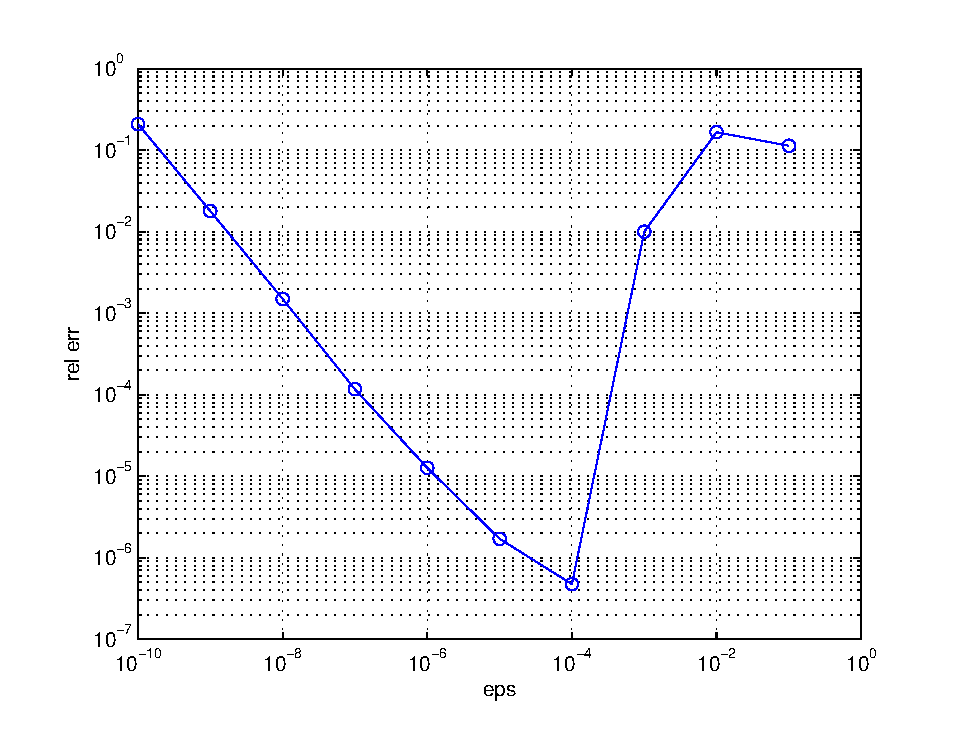
\includegraphics[width=0.6\linewidth]{Fig/err_sc}
  \end{figure}
\end{frame}

%------------------------------------------------------------------------------

\begin{frame}
  \frametitle{Single element airfoil optimization}
  \framesubtitle{NACA-0012, Ma = 0.5, $\alpha=2^\circ$}
  \begin{itemize}
  \item Objective: maximize lift
  \item Cubic design element 
    \begin{itemize}
    \item 8 variables for the displacement of a control node in the vertical direction
    \item 1 displacement constrained to zero to eliminate rigid translations
    \end{itemize}
  \item Second-order spatial discretization
  \item Constraint only on no self-penetration
  \end{itemize}
  \vspace{2mm}
   \begin{figure}
    \centering
    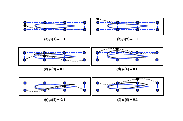
\includegraphics[width=0.65\textwidth]{Fig/nacadef}
  \end{figure}
\end{frame}

%------------------------------------------------------------------------------

\begin{frame}
  \frametitle{Single element airfoil optimization}
  \framesubtitle{NACA-0012, Ma = 0.5, $\alpha=2^\circ$}
  \begin{itemize}
  \item Optimization converges in $10$ design iterations
  \item Extreme shape deformation handled easily in the IB framework
  \end{itemize}
   \begin{columns}
    \begin{column}{0.5\textwidth}
      \begin{figure}
        \centering
        \includegraphics[width=1.0\textwidth]{Fig/naca_def}
      \end{figure}
    \end{column}
    \begin{column}{0.5\textwidth}
      \begin{figure}
        \centering
        \includegraphics[width=1.0\textwidth]{Fig/L_naca}
      \end{figure}
    \end{column}      
  \end{columns}
\end{frame}

%------------------------------------------------------------------------------

\begin{frame}
  \frametitle{Multi-element airfoil with large kinematics}
  \begin{itemize}
  \item Design of a three-element high-lift configuration
  \item Large number of design variables: geometry perturbation + 
        large displacements and deflections of the slat and flap elements
  \item Maximize the lift by finding the best position of the slat and flap
    elements without introducing any shape modification
  \item Starting from completely closed configuration, let the optimizer find 
    the best relative positions of the airfoil elements
  \end{itemize}
  \begin{figure}
    \centering
    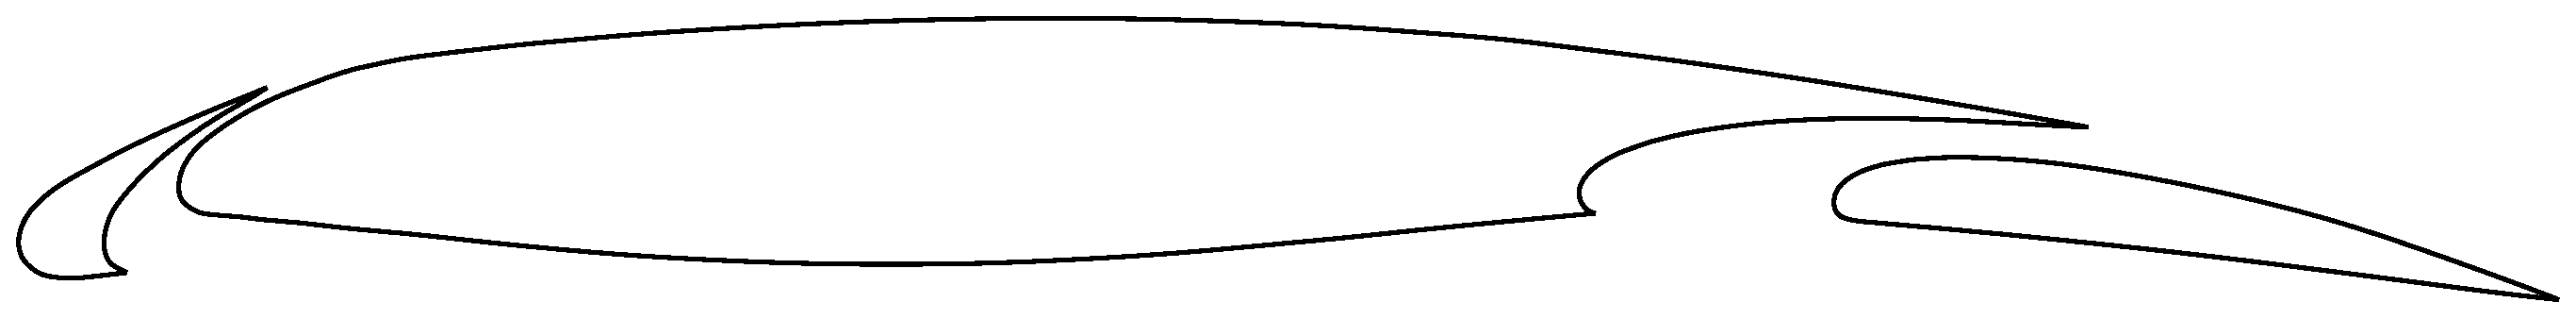
\includegraphics[width=0.8\textwidth]{Fig/L1T2_halfopen}
  \end{figure} 
\end{frame}

%------------------------------------------------------------------------------

\begin{frame}
   \frametitle{Multi-element airfoil with large kinematics}
    \begin{itemize}
    \item 6 design variables: rotation, vertical and horizontal displacements of the
      slat and flap 
    \item Pinball algorithm used to detect contacts between elements and
      avoid interpenetration
    \item Same fluid grid used to perform the previous test case
    \item $Ma = 0.2$ and $\alpha = 10^\circ$
    \item Final value of the lift doubles after 6 optimization iterations
    \end{itemize}
    \begin{figure}
      \centering
      \includegraphics[width=0.8\textwidth]{Fig/L1T2_dep}
     \end{figure}
\end{frame}

\begin{frame}
   \frametitle{Deployment of the multi-element airfoil}
  \begin{center}
    \resizebox{0.9\textwidth}{!}{%
    \animategraphics[autoplay,loop]{10}{Fig/animation}{1}{14}
  }
  \end{center}
\end{frame}

%------------------------------------------------------------------------------

\begin{frame}
\frametitle{Approximation of the viscous terms}
\begin{itemize}
\item Viscous contribution to the residual: ghost points
\begin{figure}[!ht]
  \centering
  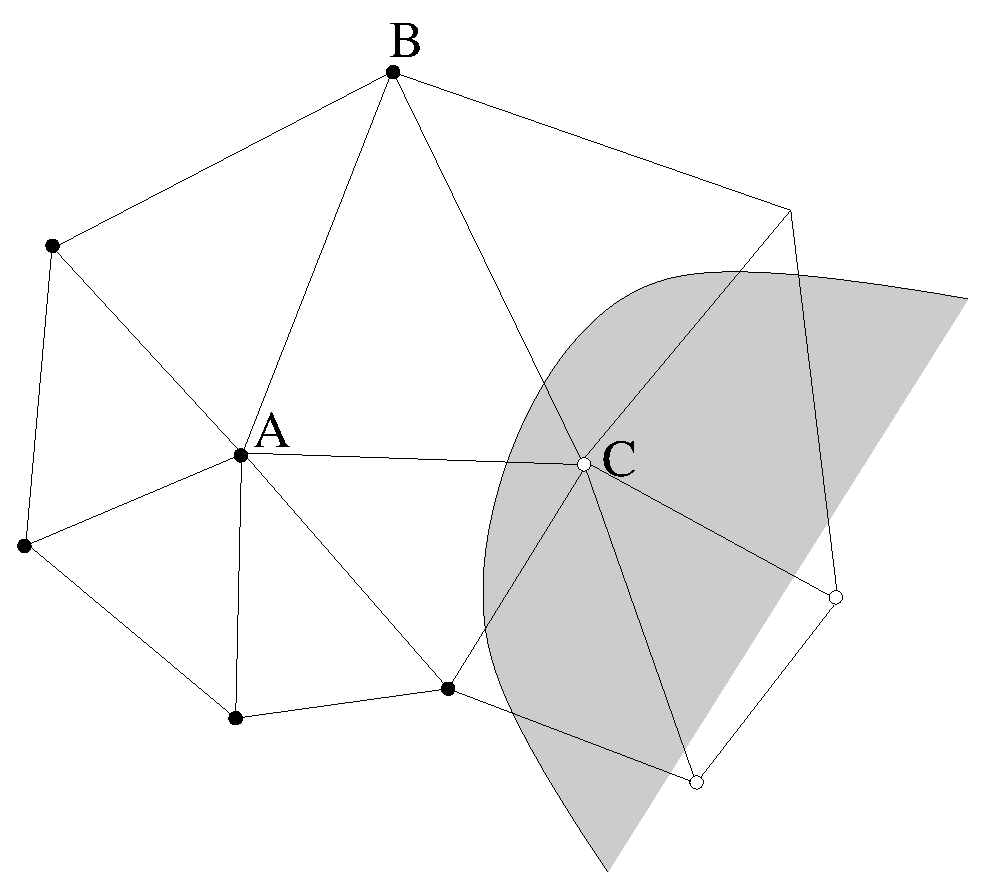
\includegraphics[width=0.35\linewidth]{Fig/GhostFEM_e}
\end{figure}
\begin{equation*}
\int_{\Omega_e}\nabla \psi_i \cdot \Fbold^v(\wbold_h, \nabla \wbold_h) \approx
|\Omega_e| \nabla \psi_i^{\Omega_e} \cdot \Fbold^v(\bar{\wbold}^{\Omega_e}_h, \nabla \wbold^{\Omega_e}_h)
\end{equation*}
\begin{equation*}
\nabla \wbold^{\Omega_e}_h = \sum_{k=1}^{N_n} \nabla \psi_k^{\Omega_e} \, \wbold_k^{\Omega_e}
\end{equation*}
\item Viscous flux depends only on the gradient of the velocity and the gradient of the temperature
\end{itemize}
\end{frame}

\begin{frame}
\frametitle{Numerical tests}
\framesubtitle{Laminar flow over a plate (Ma $=0.3$, Re $=1\,000$)}
\begin{figure}[!ht]
  \centering
  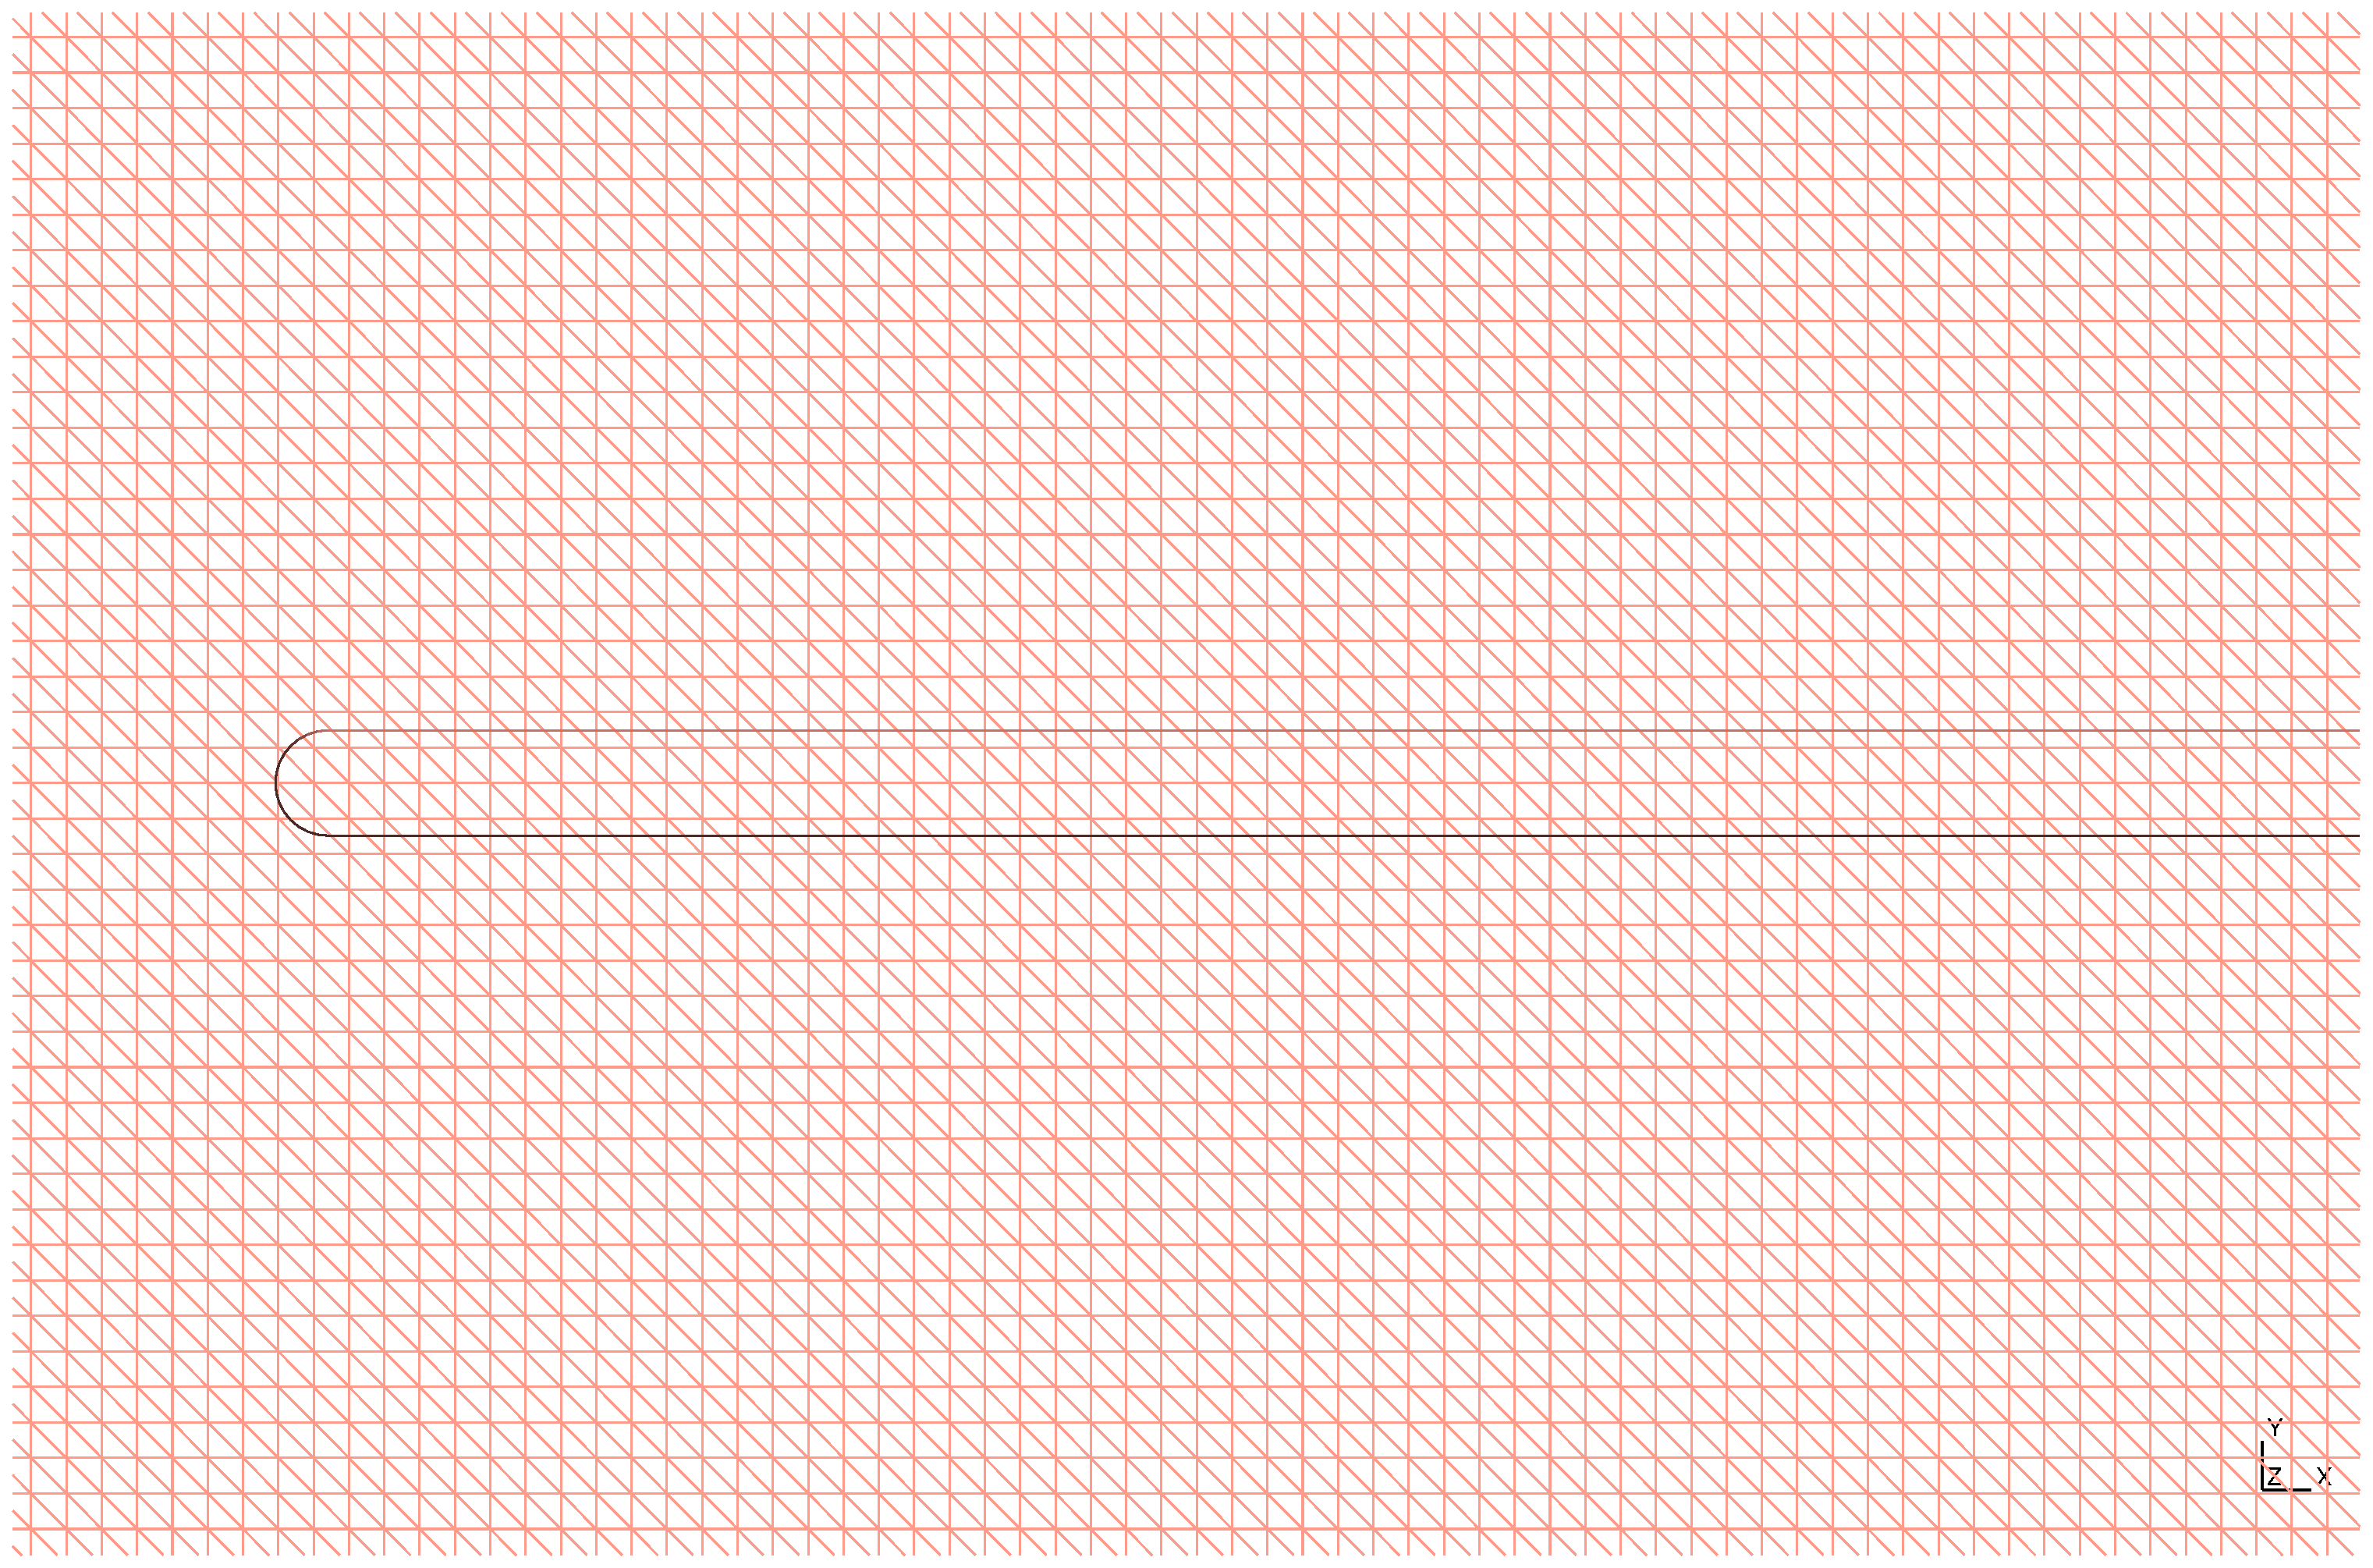
\includegraphics[width=0.47\linewidth]{Fig/gridAligned}
  \hspace{5mm}
  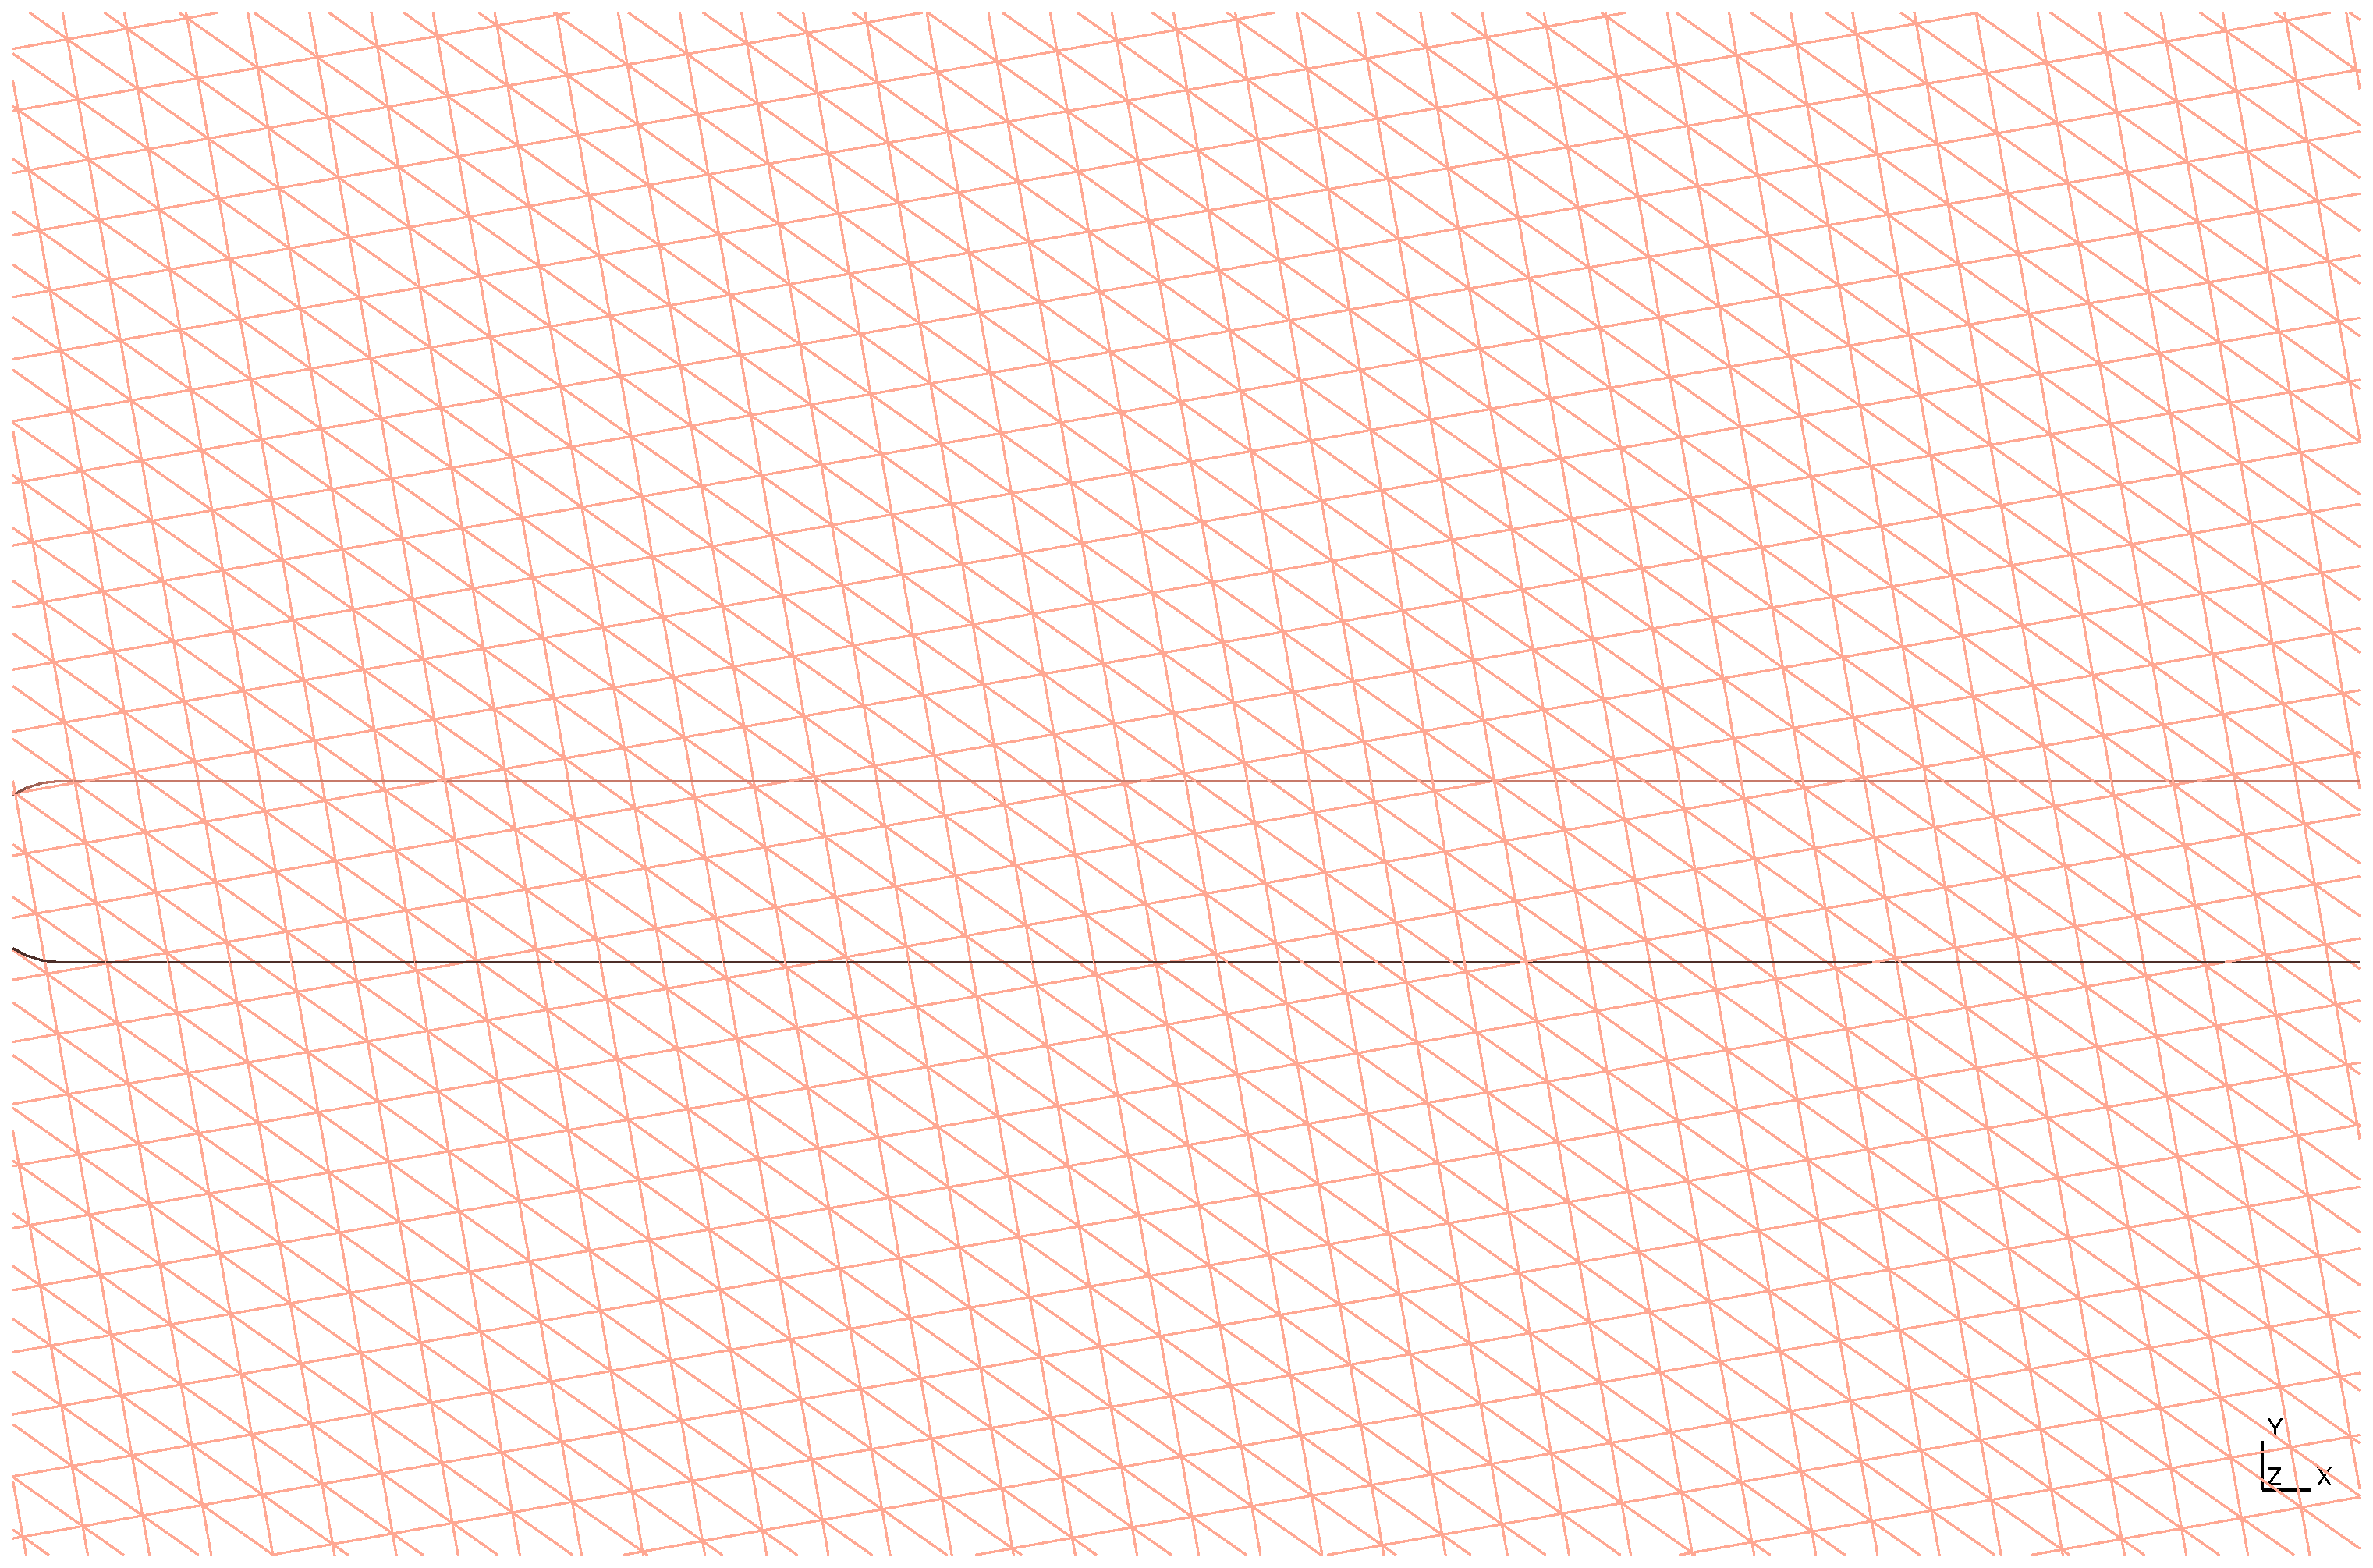
\includegraphics[width=0.47\linewidth]{Fig/gridRotated}
\end{figure}
\end{frame}

\begin{frame}
\frametitle{Numerical tests}
\framesubtitle{Laminar flow over a plate (Ma $=0.3$, Re $=1\,000$)}
\begin{figure}[!ht]
  \centering
\includegraphics[width=0.65\linewidth]{Fig/CF_alignedVsRotated}
\end{figure}
\end{frame}

%------------------------------------------------------------------------------

\begin{frame}
\frametitle{RANS}

Fluid stress
\begin{align*}
\fluidstress_{ij}&=2 \nut \left( \bar{S}_{ij}-\frac{1}{3} \pdfrac{\bar{v}_k}{x_k} \delta_{ij} \right) - \cancelto{0}{\frac{2}{3}\bar{\dens}k\delta_{ij}} \\
&\bar{S}_{ij}=\frac{1}{2}\left( \pdfrac{\bar{v}_i}{x_j}+\pdfrac{\bar{v}_j}{x_i} \right) \\
&k=\frac{1}{2} \left( \fluc{v_i}\fluc{v_i} \right)
\end{align*}

Additional transport equation
\begin{align*}
\pdfrac{~}{t}\left( \bar{\dens} \nu^{\star}\right) + \pdfrac{~}{x_j}\left( \bar{\dens}\bar{v}_j \nu^{\star} \right) = 
\frac{1}{\sigma}\left[ \pdfrac{~}{x_j} \left( \bar{\dens}(\nu+\nu^{\star})\pdfrac{\nu^{\star}}{x_j} \right) + c_{b2} \bar{\dens}(\pdfrac{\nu^{\star}}{x_j}\pdfrac{\nu^{\star}}{x_j})\right]+\nonumber\\
c_{b1}(1-f_{t2}) S^{\star} \bar{\dens}\nu^{\star}-\bar{\dens}(c_{w1}f_{w}-\frac{c_{b1}}{\kappa^2} f_{t2})
\left(\frac{\nu^{\star}}{d}\right)^{2}
\end{align*}
\end{frame}
